\section{Mathematical Modelling}

\begin{questions}

\question[1E]
Please define the values for $l$, $m$, and $t_s$ that you will use for your coursework.

\begin{solution}
   \begin{align*}
   l &= 13m  \\
   m &= 12kg \\
   t_s &= \frac{2000}{250} = 8s
   \end{align*}
\end{solution}

\question[1E]
Now derive the transfer function, $H(s) = \frac{\Theta(s)}{T(s)}$, of the Segway in terms of $l$, $m$ and $g$.

\begin{solution}
   The governing equation for the Segway is a second-order differential equation
   \begin{equation*}
   \frac{g}{l}\theta(t) + torque(t) = m\frac{d^2}{dt^2}\theta(t)
   \end{equation*}

   Take the Laplace Transform
   \begin{equation*}
   \frac{g}{l}\Theta(s) + T(s) = m(s^2\Theta(s) - s\Theta(0^-) - \dot{\Theta}(0^-))
   \end{equation*}

   Assuming $\Theta(0^-)$ and $\dot{\Theta}(0^-)$ equals zerod (WHY?), the equation becomes
   \begin{equation*}
   \frac{g}{l}\Theta(s) + T(s) = ms^2\Theta(s)
   \end{equation*}

   In order to obtain the transfer function of the Segway, $H(s)$, which equals $\frac{\Theta(s)}{T(s)}$, one side of the equation needs to be rearrange into the form $\frac{\Theta(s)}{T(s)}$
   \begin{equation*}
   \frac{\Theta(s)}{T(s)} = \frac{1}{ms^2-\frac{g}{l}}
   \end{equation*}

   Hence, the transfer function is
   \begin{equation}\label{eq:TF_of_Segway}
   H(s) = \frac{1}{ms^2-\frac{g}{l}}
   \end{equation}
\end{solution}

\question[1E]
Using your values for $l$ and $m$ along with $g=3.711 ms^{-2}$, write the transfer function with the denominator and numerator of your transfer function in polynomial form.

\begin{solution}
   Subsituting the value of $l$, $m$, and $g$ into the transfer function (\ref{eq:TF_of_Segway})
   \begin{equation}\label{eq:TF_of_Segway_with_values}
   H(s) = \frac{1}{12s^2-\frac{3.711}{13}}
   \end{equation}
\end{solution}

\question[1E]
Calculate the position of the poles for your Segway and plot the poles on the complex plane.

\begin{solution}
   The poles is the roots of the denominator of the transfer function (\ref{eq:TF_of_Segway_with_values})
   \begin{align*}
   12s^2-\frac{3.711}{13} &= 0 \\
   s &= \pm\sqrt{\frac{3.711}{13\times12}}
   \end{align*}

   Using MATLAB to plot the poles on the complex plane
   \begin{minted}[fontsize=\small, xleftmargin=-20pt]{matlab}
   num = 1;
   den = [12 0 -3.711/13];
   H = tf(num, den)
   pzmap(H)
   \end{minted}
   \begin{minipage}[htbp]{\linewidth}
      \centering
      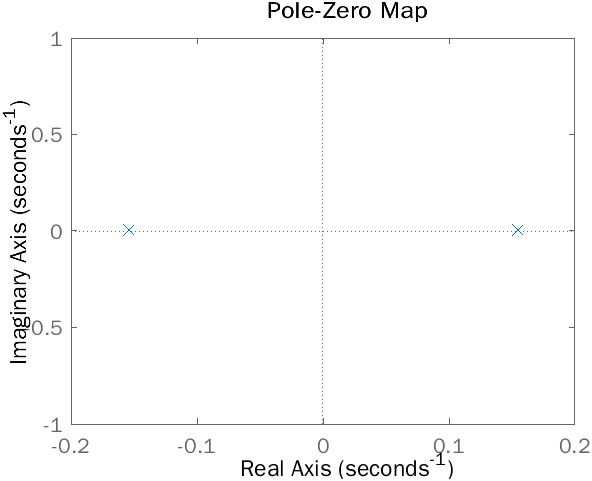
\includegraphics[scale=0.8]{figures/D.png}
      \captionof{figure}{Poles of $H(s)$ on the complex plane}
      \label{fig:poles_of_H}
   \end{minipage}
\end{solution}

\setcounter{lastquestioncounter}{\value{question}}
\end{questions}
